\begin{problem}{43/figs/pic.jpg}{Coloring the Map of Iran}This is one of the most important problems in the history of graph theory:
	
What is the minimum number of colors needed to color the provinces of Iran so that no two neighboring provinces have the same color?

\textbf{Additional problems}:
\begin{itemize}
\item What is the size of the largest subset of Iranian provinces that can be colored with 3 colors so that no two neighboring provinces have the same color?
\item Question 1, but what about 2 colors?
\item Question 1, but what about 1 color?
\end{itemize}
(link to the map:  \url{https://skilledup.ir/iran-map/)}

\begin{center}
	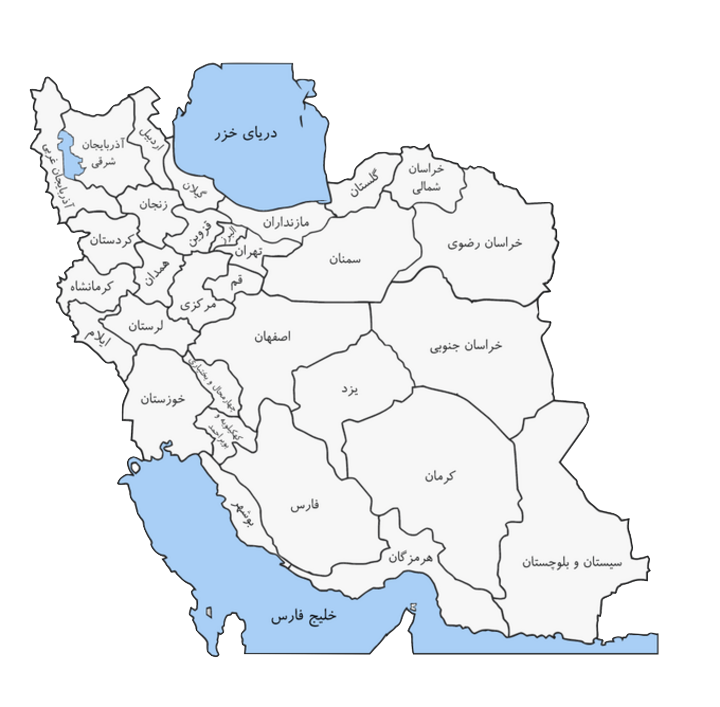
\includegraphics[width=9cm]{43/figs/43_iran.png}
\end{center}

 Link to the problem on Twitter: \url{https://twitter.com/Riazi_Cafe/status/1707280079318098026}\end{problem}